\documentclass[12pt, border = 8pt, varwidth, convert]{standalone}

% TikZ
\usepackage{tikz}
\usetikzlibrary{calc}% 计算库
\usetikzlibrary{arrows.meta}% 箭头库
\usetikzlibrary{positioning}

\begin{document} %在document环境中撰写文档

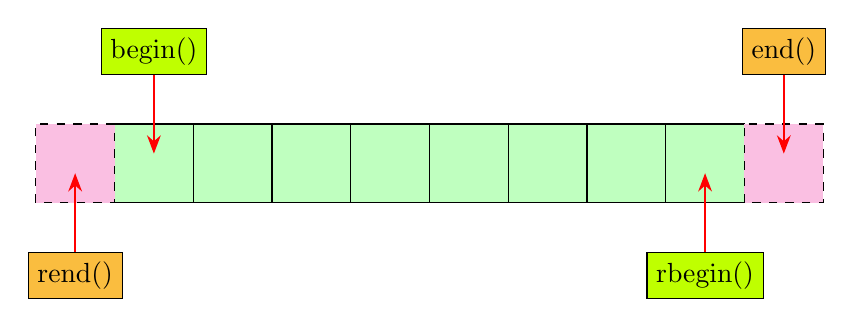
\begin{tikzpicture}[x=1.0cm, y=1.0cm]
  % 循环布置命名坐标
  \foreach \x in {0,1,...,9}
  {
    \node[inner sep=1pt] (BL\x) at (\x, 0) {};% 左下角
    \node[inner sep=1pt] (UR\x) at (\x+1, 1) {};% 右上角
    \node (MM\x) at ($(BL\x)!0.5!(UR\x)$) {};% 对角线中点
  }
  % 循环绘制数组矩形
  \foreach \x in {1,2,...,8}
  {
    \draw[fill=green!25] (BL\x) rectangle (UR\x);% 使用命名坐标
  }
  % 迭代器结束虚线框
  \draw[fill=magenta!25, dashed] (BL0) rectangle (UR0);
  \draw[fill=magenta!25, dashed] (BL9) rectangle (UR9);
  % 正向迭代器开始位置
  \node[fill=green!25!yellow, draw, above=1.0 of MM1] (note1) {begin()};
  % 正向迭代器结束位置 
  \node[fill=magenta!25!yellow, draw, above=1.0 of MM9] (note2) {end()};
  % 反向迭代器结束位置
  \node[fill=magenta!25!yellow, draw, below=1.0 of MM0] (note3) {rend()};
  % 反向迭代器开始位置
  \node[fill=green!25!yellow, draw, below=1.0 of MM8] (note4) {rbegin()};
  % 绘制指示线
  \draw[-{Stealth[scale=1.0]}, red, thick] (note1.south) -- (MM1.north);
  \draw[-{Stealth[scale=1.0]}, red, thick] (note2.south) -- (MM9.north);
  \draw[-{Stealth[scale=1.0]}, red, thick] (note3.north) -- (MM0.south);
  \draw[-{Stealth[scale=1.0]}, red, thick] (note4.north) -- (MM8.south);        
\end{tikzpicture}
\end{document}

%%% Local Variables:
%%% mode: latex
%%% TeX-master: t
%%% End:
